\documentclass[11.5pt]{sig-alternate} % sets document style to sig-alternate
% packages
% typesetting
%\usepackage{dirtytalk} % typset quotations easier (\say{stuff})
\usepackage{hanging} % hanging paragraphs
\usepackage[defaultlines=3,all]{nowidow} % avoid widows
\usepackage[pdfpagelabels=false]{hyperref} % produce hypertext links, includes backref and nameref
\usepackage{xurl} % defines url linebreaks, loads url package
\usepackage{microtype}
%\usepackage[super]{nth} % easily create superscript ordinal numbers with \nth{x}
\usepackage{textcomp}
\newcommand{\texttildemid}{\raisebox{0.4ex}{\texttildelow}}
% layout
%\usepackage{enumitem} % control layout of itemize, enumerate, description
\usepackage{fancyhdr} % control page headers and footers
\usepackage{float} % improved interface for floating objects
%\usepackage{multicol} % intermix single and multiple column pages
% language
\usepackage[utf8]{inputenc} % accept different input encodings
\usepackage[english]{babel} % multilanguage support
% misc
\usepackage{graphicx} % builds upon graphics package, \includegraphics
%\usepackage{lastpage} % reference number of pages
%\usepackage{comment} % exclude portions of text (?)
\usepackage{xcolor} % color extensions
\usepackage[backend=biber, style=apa]{biblatex} % sophisticated bibliographies % necessary for HTML to display author info and date on abstract page
\usepackage{csquotes} % advanced quotations, makes biblatex happy
\usepackage{authblk} % support for footnote style author/affiliation
% tables and figures
\usepackage{tabularray}
%\usepackage{array} % extend array and tabular environments
\usepackage{caption} % customize captions in figures and tables (rotating captions, sideways captions, etc)
%\usepackage{cuted} % allow mixing of \onecolumn and \twocolumn on same page
\usepackage{multirow} % create tabular cells spanning multiple rows
%\usepackage{subfigure} % deprecated, support for manipulation of small figures
%\usepackage{tabularx} % extension of tabular with column designator "x", creates paragraph-like column whose width automatically expands
%\usepackage{wrapfig} % allows figures or tables to have text wrapped around them
%\usepackage{booktabs} % better rules
% dummy text
%\usepackage{blindtext} % blind text dummy text
%\usepackage{kantlipsum} % Kant style dummy text
\usepackage{lipsum} %lorem ipsum dummy text
% other helpful packages may be booktabs, longtable, longtabu, microtype

\pagestyle{fancy} % sets pagestyle to fancy for fancy headers and footers

% header and footer
% modern way to set header image
\renewcommand{\headrulewidth}{0pt} % defines thickness of line under header
\renewcommand{\footrulewidth}{0pt} % defines thickness of line above header
\setlength\headheight{80.0pt} % sets height between top margin and header image, effectively moves page contents down
\addtolength{\textheight}{-80.0pt} % seems to affect the lower height. maybe only works properly if footer numbers enabled?
\fancyhf{}
\fancyhead[CE, CO]{
\includegraphics[width=\textwidth]{headerImage.png}}
% footer
%\fancyfoot[LE,LO]{Article Title Here \\ DOI: }% left footer article title and doi
%\fancyfoot[CE,CO]{{}} % center footer empty
%\fancyfoot[RE,RO]{\thepage} % right footer page numbers
%\pagenumbering{arabic} % arabic (1, 2, 3) numbering in footer

\hypersetup{colorlinks=true,urlcolor=blue} % sets link color to blue
\urlstyle{same} % sets url typeface to same as rest of text

% set caption and figure to italics, label bold, left align captions, does not transfer to HTML
\captionsetup{labelfont=bf, font={large, it}, justification=raggedright, singlelinecheck=false}
\renewcommand\theContinuedFloat{\alph{ContinuedFloat}}

%this next bit is confusing, but essentially changes the width of the abstract. Seems to have been copied from this https://tex.stackexchange.com/questions/151583/how-to-adjust-the-width-of-abstract
\let\oldabstract\abstract
\let\oldendabstract\endabstract
\makeatletter %changes @ catcode to enable modification (in parsep)
\renewenvironment{abstract} %alters the abstract environment
{\renewenvironment{quotation}%
               {\list{}{\addtolength{\leftmargin}{1em} % change this value to add or remove length to the the default ?
                        \listparindent 1.5em%
                        \itemindent    \listparindent%
                        \rightmargin   \leftmargin%
                        \parsep        \z@ \@plus\p@}%
                \item\relax}%
               {\endlist}%
\oldabstract}
{\oldendabstract}
\makeatother %changes @ catcode to disable modification

% checks
% italics -
% links -
% dashes
% tildes
\begin{document}

\title{Teaching Science through Inquiry Based Field Experiences
Using Orientation and Mobility}

\author[1]{\large \color{blue}Danene Fast}
\author[1]{\large \color{blue}Tiffany Wild}
\affil[1]{The Ohio State University}

\toappear{}
%% ABSTRACT
\maketitle
\begin{@twocolumnfalse} 
\begin{abstract}
\item 
\textit {Instruction in science can be difficult for students with visual impairments due to the use of visual instruction that is often used for conceptual understanding. Pedagogical approaches to teaching science continue to evolve, with inquiry-based science instruction as a primary instructional method used in current classrooms.In teaching students with visual impairments, inquiry is a strategy that has been traditionally been used in orientation and mobility (O\&M) instruction, in an effort to teach students with vision loss to explore and make conclusions about their environments through the use of all senses. The purpose of this review is to outline how orientation and mobility (O\&M) lessons can reinforce early science concepts for students who are blind or visually impaired through inquiry based experiences}
\\ \\
Keywords: inquiry, visual impairments, orientation and mobility, conceptual development
\end{abstract}
\end{@twocolumnfalse}

%% AUTHOR INFORMATION

\textbf{*Corresponding Author, Danene Fast}\\
\href{mailto: fast.40@osu.edu }{(fast.40@osu.edu)} \\
\textit{Submitted  Jan 22 2018 }\\
\textit{Accepted Jun 18 2018} \\
\textit{Published online October 11th, 2018} \\
\textit{DOI: 10.14448/jsesd.10.0003} \\
\pagebreak
\clearpage

\begin{large}
\section*{SCIENCE AND STUDENTS WITH DISABILITIES}

The Individuals with Disabilities Education Improvement Act (IDEA) 20 U.S.C. § 1400(c)(d) (2004) states that improving educational results for children with disabilities is an essential element of national policy that ensures equality of opportunity.  Of the approximately 100,000 students with visual impairments throughout the United States, few of them fully participate in science instruction within their school settings (Beck-Winchatz \& Riccobono, 2007).  The National Science Teachers Association (NSTA) recognizes that, even with the best of intentions, barriers to learning science are present and, as a result, issued a position statement to address inclusion of students with disabilities (National Science Teachers Association (NSTA), 2004).

Using guidelines from IDEA and the national science education standards published through the Next Generation Science Standards (NGSS) (2013), NSTA’s position paper includes a number of recommendation topics to ensure students with disabilities are integrated into science. These recommendations include:  (a) use of strategies to overcome educational and physical barriers, (b) selection of science curriculum to promote accessibility and inclusiveness of people with disabilities, (c) development of assessment tools that are accessible for all students, (d) use of collaboration to overcome attitudinal barriers about what is involved in teaching students with disabilities, and (e) promotion of science and science-related careers for students with disabilities (NSTA, 2004).

One specific area addressed within the NSTA position paper, under the topic of collaboration, includes ensuring accessibility for students with a variety of disabilities by working with school staff to ensure that teachers are prepared to help students master the science content (NSTA, 2004).  All educators, including professionals such as orientation and mobility specialists who work with students who are blind or visually impaired, should be accountable to this standard (Smith, 2006).  With creativity, collaboration, and review of concepts being taught across disciplines, the field of orientation and mobility (O\&M) can provide experiences that help students with vision loss to develop a conceptual framework for science concepts.

\section*{SPECIALIZED NEEDS OF STUDENTS WITH VISUAL IMPAIRMENTS}

Research has found that general education teachers are not prepared to teach students with visual impairments (Norman, Caseu, \& Stefanich, 1998; Kahn \& Lewis, 2014) while teachers of students with visual impairments are ill-prepared to teach science, technology, engineering, and mathematics (STEM) content (Kapperman, Heinz \& Sticken, 2000).  Therefore, there is a divide in order to meet the needs of students with visual impairments.  However, if content experts work together with the specialists who provide services to students with visual impairments, all involved with the educational process will benefit.  The students will get the content delivered in an accessible manner while the general education teacher, in this case the science teacher, can benefit from collaborating with an expert who recognizes and addresses the needs of students with visual impairments.  

Because much of what is learned within classroom settings is visual, specialized adaptations are used to educate students with vision loss.  Students with visual impairments have unique needs that stretch beyond those of other low incidence populations, including competency skills sets that go beyond the core materials developed for students within general education.  Under the law, the IDEA mandates that functional outcomes, as well as academic outcomes, are addressed in every individualized education program (IEP) for students categorized within special education (IDEA, 2004).  In addition to addressing the demands of a “typical” educational curriculum, administrators and IEP team members serving students with visual impairments must also consider accommodations that address access to the expanded core curriculum (ECC).
	
 First formulated by Hatlen (1996), the expanded core curriculum (ECC) is an established set of specialized skills for students with visual impairments.  It was established because students with vision loss are unable to observe the non-verbal behaviors and actions of others, affecting the manner in which incidental skills are learned (Allman \& Lewis, 2014).  Designed to go beyond the core components of math, reading, writing, and science to address essential areas and experiences that are unique to persons who are visually impaired (Lohmeier, Blankenship, \& Hatlen, 2009; Pugh \& Erin, 1999), the ECC addresses functional outcomes for students with visual impairments. O\&M is one section of the ECC that addresses the ability to move about in home, school, and community settings. Skills within the O\&M curriculum are ideally taught by certified specialists trained in the discipline of orientation and mobility, who work closely with parents and school professionals to adapt environments and support student learning across settings (Cmar, Griffin-Shirley, Kelley, \& Lawrence, 2015).
 
\section*{WHAT IS ORIENTATION \& MOBILITY?}

O\&M is a related service provided to students with vision loss in school settings by specialists who are trained to teach skills associated with O\&M; these skill sets are addressed through the individualized education plan (IEP).  Orientation and mobility specialists focus on two components of learning: (a) knowing one’s position in space and keeping track of how position changes with movement and (b) the physical act of traveling from one place to another.  Through concepts associated with these components, individuals who are visually impaired are taught to travel safely, efficiently, independently, and gracefully as possible (Ambrose-Zaken, Calhoon, \& Keim, 2010). 
	
While O\&M is a part of the ECC and, the ECC is “designed to go beyond the core components of math, reading, writing, and science,” there is crossover that can be established between the disciplines of O\& M and science.  Components of the O\&M curriculum can be naturally incorporated into science curriculum reflective of NGSS and can be taught in collaboration with the general education teacher (Sapp \& Hatlen, 2010).  By examining O\& M curriculum and texts (Blasch, Wiener, \& Welsh, 2010; Progrund, et. al, 2012), one can identify many science concepts that can be reinforced through O\& M instruction (Smith, 2006).
 
\section*{USING INQUIRY BASED INSTRUCTION FOR SCIENCE AND O\&M}

Inquiry can be defined as diverse ways of studying the natural world in order to develop knowledge and understanding of science concepts (National Research Council, 1996).  This approach to learning has emerged as a prominent technique used to teach science in general education settings (Maroney, Finson, Beaver, \& Jensen, 2003; Rizzo \& Taylor, 2016; Scruggs, et al., 1993; Scruggs \& Mastropieri, 2007).  The use of relevant experiences – including connections between the daily experience of students and what they are learning – is one way to help children make sense of their natural world within inquiry-driven methods.  

Samarapungavan and colleagues (2015) state that engaging students in mindful, inquiry-driven, modeling activities helps students to understand dimensions of science.  Through the use of inquiry methods for learners of all levels, instruction is aimed at developing the skills and knowledge needed within given situations, through meaningful interactions.  In these methods, a socially negotiated process emphasizes the importance of using contextualized approaches within inquiry to impact student learning (Boyd \& Richerson, 2005; Samarapungavan, Tippins, \& Bryan, 2015).

Inquiry-based instruction has been found to beneficial to students with disabilities (Lynch, S., Taymans, J., Watson, W., Ochesendorf, R., Pyke, C., \& Szesze, M., 2007).  Mastropieri (2005) reported that behavioral problems in the classroom lessened as a result of inquiry-based teaching methods being used in the classroom.  Wild and Paul (2012) found that 61.1\% of the science classrooms which included students with visual impairments were using inquiry-based science methods as part of instruction.  
	
 Contextualized approaches to learning are also appropriate for students who are blind or visually impaired, as research has shown that students with visual impairments have considered science a difficult subject because of the reliance on visual instruction for the teaching of concepts (Jones, Minogue, Oppewal, Cook, \& Broadwell, 2006; Penrod, Haley, \& Matheson, 2005; Sahin \& Yorek, 2009; Wild, Hilson, \& Farrand, 2014).  Use of inquiry-based instructional methods used in science are effective for students with visual impairments (Erwin, et. al., 2001; Wild \& Paul, 2012; Wild \& Trundle, 2010a; 2010b).  Activity-focused, inquiry-based instruction techniques can facilitate the efforts of teachers and specialists in making appropriate modifications based upon individualized needs of students (Wild \& Paul, 2012).
 
In a further analysis of inquiry-based teaching methods for students with visual impairments, it was noted there is a dearth of research.  Inquiry-based instructional methods have been found to be beneficial to students with visual impairments but have only been analyzed in teaching concepts of scale, environmental science, seasonal change, space, sound, geoscience, and biodiversity to students with visual impairment (Jones, Taylor, \& Broadwell, 2008; Rule, 2011; Wild \& Trundle, 2010a; 2010b; Wild, Hobson, \& Hilson 2012; Wild, Hilson, \& Farrand, 2014; Hilson, Hobson, \& Wild, 2016).  While analyzing field-based inquiry teaching, it was found that inquiry-based methods were beneficial in helping students overcome scientific misconceptions while still holding onto misconceptions of science concepts that were unique to those with visual impairments (Wild, Hobson, \& Hilson 2012; Wild, Hilson, \& Farrand, 2014; Hilson, Hobson, \& Wild, 2016).  One study, directly used the help of orientation and mobility (O\&M) instructors to support the inquiry-based learning that occurred in field-based geoscience (Wild, Hilson, \& Farrand, 2014).  The O\&M instructors directly supported the content-instructions by helping students orient to different geologic phenomena such as caves, caverns, and fossil-rich sites in order to assist in navigation and to help students fully engage in the numerous field-based experiences with their peers. 

While an effective strategy for science education, inquiry can also be a key pedagogical strategy in teaching O\&M; one that allows students to explore and make conclusions about their environments, through the guidance of an orientation and mobility specialist. In teaching students with visual impairments within general education settings, using a crossover of concepts between O\&M and science – including a crossover of instructional strategies, such as inquiry-based education, can facilitate conceptual development.

\section*{O\&M CONNECTIONS TO SCIENCE}

\subsection*{Forces and Interactions}

Students who are blind or visually impaired must use a sense of touch to discover properties of their immediate surroundings; teaching students to use their sense of touch to meaningfully interact with environments is one aspect of O\&M training. Loomis and Lederman (1986) point out that touching involves detecting relative positions and movements of parts of the body (Guth, Rieser, \& Ashmead, 2010). In order to become independent travelers, students who are blind or visually impaired must experience environments through touch, recognizing how the proprioceptive integration of touch and movement in determines position in space. Integration of scientific concepts of physical interactions and analysis of these interactions in relation to force, students with vision loss can connect concepts across disciplines.
	
Beginning with basic science skills, such as \textit{investigations that compare effects of different strengths or different directions of pushes and analysis of data to determine if design solutions can change the speed or direction of an object} (NGSS, 2013, p. 4), O\&M activities can be used in elementary lessons to reinforce these objectives.  With minimal creativity and collaboration between classroom teachers and O\&M instructors, lessons that address recognition of landmarks and clues for orientation purposes, basic spatial awareness, directional/positional concepts, and time-distance concepts can also reinforce scientific concepts of forces and interactions.
	
For example, exploration of forces and interactions can be done on a playground (Fast \& Wild, 2018).  By taking the lesson outside, students can engage in inquiry-based experiences from the classroom to the playground to address science and engineering practices. While the science teacher focuses on push and pull with different strengths and directions, ability to change speed or direction, and concepts of bigger pushes or pulls making things speed up or slow down, the O\&M specialist can focus on discussion of relationships between the student and the environment with focus on the push and pull of the long cane, typically used by students with visual impairments (Fast \& Wild, 2018). The O\&M instructor can work with the science teacher to help students identify what happens when objects are pushed or pulled, forces that interact within the environment, and how to “measure” the forces needed to speed up or slow down an object in motion.
 
\begin{figure}[h]
    \centering
    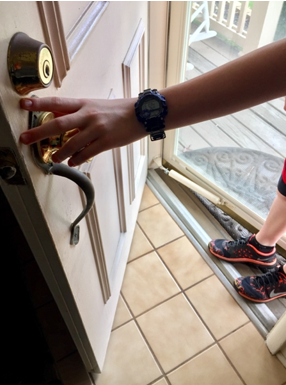
\includegraphics[width=0.6\linewidth]{fig1.png}
    \caption{Forces and Motion: Push and Pull}
\end{figure}

\subsection*{Habitat}

Within O\&M training, spatial updating and frames of reference within environments are two fundamental concepts important in understanding spatial orientation (Long \& Giudice 2010).  O\&M lessons that address environmental travel skills – including residential, urban, rural, and suburban environments, navigation within these settings, and use of cardinal directions to maintain orientation can also reinforce scientific concepts of habitat and how the environments are changed to address the needs of pedestrians (Hilson, Hobson, \& Wild, 2016).

NGSS standards addressing the concept of habitats state that to demonstrate mastery, \textit{students must construct arguments, supported by evidence, for how plants and animals can change the environment to meet their needs} (NGSS, 2013, p. 7).  Allowing students with vision loss who are already participating in O\&M lessons within varied community settings to expand their conceptual knowledge by using inquiry based learning within these settings can improve O\&M concepts of environmental awareness and mental mapping skills while solidifying core science concepts (Hilson, Hobson, \& Wild, 2016).
	
 For example, students can engage in inquiry-based experiences in the outdoors by examining plants and animals in their natural environments, allowing for authentic experiences that are vitally important to the conceptual understanding of students with visual impairment. While the science teacher encourages examination of plants and animals in their natural environment and evidence for how these plants and animals can change their environment to meet their needs, the O\&M instructor can assist by helping students use their senses to observe characteristics of the natural world within environments where travel skills are being taught.  Similar to the research conducted by Hilson, Hobson, and Wild (2016), the O\&M instructor can support learning within field-based experiences, such as conversation parks, wildlife centers, zoos and aquariums, or field stations.  The O\&M instructor can provide tactile maps, guidance in directional concepts, and help in navigation of complex terrain using modified travel skills and equipment all while ensuring students are fully engaged in the science instruction happening in these new environments.  Specific to students with visual impairments, the O\&M instructor’s curriculum describes how they need to prepare students to explore and predict naturally occurring patterns that can impact travel, such as plants and tree roots.  This requirement naturally aligns with the science standards of observing and describing patterns in the natural world, allowing the science teacher and O\&M instructor to co-teach these concepts.
 
\begin{figure}[h]
    \centering
    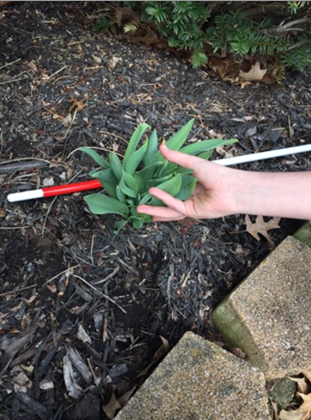
\includegraphics[width=0.8\linewidth]{fig2.png}
    \caption{Habitat}
\end{figure}

\section*{CONCLUSION}

“All educators, including professionals such as orientation and mobility specialists who work with students who are blind or visually impaired, should be accountable to educational standards” (Smith, 2006, p. 161).  Inquiry based instructional methods across the disciplines of science and O\&M can provide a number of hands-on experiences for students with vision loss, allowing students opportunity to investigate, explore, problem solve, and integrate scientific concepts into supervised travel routines. Through the use of collaboration between the science teacher and the O\&M instructor, students who are blind or visually impaired can be provided with opportunities that imbed science concepts into O\&M training, providing an inclusive curriculum across disciplines and unique opportunities for learning.

\end{large}
\clearpage
\section*{REFERENCES}\par 

\leftskip 0.25in
\parindent -0.25in 

Allman, C. \& Lewis, S., Eds. (2014). \textit{ECC Essentials: Teaching the Expanded Core Curriculum to Students with Visual Impairments}. AFB Press:  New York, NY.

Ambrose-Zaken, G., Calhoon, C. \& Keim, J. (2010). Teaching orientation and mobility to students with cognitive impairments and vision loss.  In W. R. Wiener, R. L. Welsh, \& B. B. Blasch (Eds.), Foundations of orientation and mobility, Volume 2, Instructional strategies and practical applications (3rd ed.) (pp. 420-461). New York:  American Foundation for the Blind.

Beck-Winchatz, B. \& Riccobono, M. (2008). Advancing participation of blind students in science, technology, engineering, and math. \textit{Advances in Space Research, 42}, 1855-1858.

Blasch, B., Wiener, W., \& Welsh, R. (Eds). (2010). \textit{Foundations of orientation and mobility, Volumes I \& II} (3rd Ed.). New York:  American Foundation for the Blind.

Boyd, R., \& Richerson, J. (2005). Solving the puzzle of human cooperation. In S. Levinson \& N. Enfield (Eds.), \textit{Evolution and culture} (pp. 105-132). Cambridge, MA: MIT Press.

Cmar, J. L., Griffin-Shirley, N., Kelley, P., \& Lawrence, B. (2015). \textit{The role of the orientation and mobility specialist in public schools}.  Position paper of the Division on Visual Impairments and Deafblindness, Council for Exceptional Children. Arlington, VA:  Council for Exceptional Children.

Erwin, E., Perkins, T., Ayala, J., Fine, M., \& Rubin, E. (2001). You don’t have to be sighted to be a scientist, do you? Issues and outcomes in science and education.  \textit{Journal of Visual Impairment \& Blindness, 95(6)}, 338-352.

Fast, D. \& Wild, T. (2018). Traveling with science:  Working with orientation and mobility specialists to make science accessible for kindergarten students with visual impairments.  \textit{Science and Children, 55(5)}, 54-59.

Guth, D., Rieser, J., \& Ashmead, D. (2010). Perceiving to move and moving to perceive:  Control of locomotion by students with vision loss.  In W. R. Wiener, R. L. Welsh, \& B. B. Blasch 	(Eds.), \textit{Foundations of orientation and mobility:  Volume one:  History and theory} (pp.3-44).  New York, NY:  American Foundation for the Blind.

Hatlen, P. (1996). The core curriculum for blind and visually impaired students, including those with additional disabilities.  \textit{RE:view, 28(1)}, 25-32.

Hilson, M., Hobson, S., \& Wild, T. (2016). Conceptual understandings of students with visual impairments about biodiversity across ecosystems.  \textit{Journal of Blindness Innovation and Research, 6(2)}.  Retrieved from: \url{https://nfb.org/images/nfb/publications/jbir/jbir16/jbir0602tc.html}

Individuals with Disabilities Education Act (IDEA), 20 U.S.C. § 1400 (2004).

Jones, M.G., Minogue, J., Oppewal, T., Cook, M.P., \& Broadwell, B. (2006). Visualizing without vision at the microscale:  Students with visual impairments explore cells with touch. \textit{Journal of Science Education \& Technology, 15 (5/6)}, 345-351. doi: 10.1007/s10956-006-9022-6

Jones, M.G., Taylor, A., \& Broadwell, B. (2008). Concepts of scales held by students with visual impairments.  \textit{Journal of Research in Science Teaching}, 1-14.

Kahn, S. \& Lewis, A.R. (2014). Survey on teaching science to K-12 students with disabilities:  Teacher preparedness and attitudes. \textit{Journal of Science Teacher Education, 25}(8), 885-910. doi: 10.1007/s10972-014-9406-z 

Kapperman, G., Heinz, T., \& Sticken, J. (2000). Mathematics.  In A. J. Koenig and M. C. Holbrook (Eds.), \textit{Foundations of education, volume two:  Instructional strategies for teaching children and youth with visual impairments}.  New York, NY:  American Foundations for the Blind.

Lohmeier, K., Blankenship, K. \& Hatlen, P. (2009). Expanded core curriculum:  12 years later. 	\textit{Journal of Visual Impairment and Blindness, 103}(2), pp. 103-112.

Long, R. G. \& Giudice, N. A. (2010). Establishing and maintaining orientation and mobility.  In W. R. Wiener, R. L. Welsh, \& B. B. Blasch (Eds.), \textit{Foundations of orientation and mobility:  Volume one:  History and theory} (pp.3-44).  New York, NY:  American Foundation for the Blind.

Loomis, J. M., \& Lederman, S. J. (1986). Tactual perception.  In K. Boff, L. Kaufman, \& J. Thomas (Eds.), \textit{Handbook of perception and human performance.  Volume II:  Cognitive processes and performance}.  New York: Wiley. 

Lynch, S., Taymans, J., Watson, W., Ochesendorf, R., Pyke, C., \& Szesze, M.  (2007). Effectiveness of a highly rated science curriculum for students with disabilities in general education classrooms.  \textit{Exceptional Children. 73}(2), 202-223.
 
Maroney, S. A., Finson, K. D., Beaver, J. B., \& Jensen, M. M. (2003). Preparing for successful inquiry in inclusive science classrooms.  \textit{Teaching Exceptional Children, 36 (1)}, 18-25.

Mastopieri, M. (2005). Margo Mastopieri on science education and students with disabilities. In Carin, A., Bass, J., \& Contant, T. (Eds.), Teaching science as inquiry (pp. 287-288).  Upper Saddle River, New Jersey: Pearson Merrill Prentice Hall.

National Research Council (NRC). (1996). National science education standards.  Washington, DC:  National Academy Press.

National Science Teachers Association - NSTA. (2004, May). NSTA Position Statement:  Students with Disabilities. Retrieved April 22, 2017, from \url{http://www.nsta.org/about/positions/disabilities.aspx}

NGSS Lead States. (2013). Next generation science standards: For states, by states. 	Washington, DC; National Academies Press.

Norman, K., Caseau, D. L., \& Stefanich, G. (1998). Teaching students with disabilities in inclusive science classrooms: survey results. \textit{Science Education, 82}(2), 127-146.

Penrod, W., Haley, C., \& Mattheson, L. (2005). A model for improving science teaching for students with visual impairments. \textit{RE:view: Rehabilitatiton Education for Blindness and Visual Impairment, 37}(2), 53-58.

Pogrund, R., Sewell, D., Anderson, H., Calaci, L., Cowart, M.F., Gonzalez, C., Marsh, R.A., \& Roberson-Smith, B. (2012). \textit{Teaching age-appropriate purposeful skills (TAPS):  An orientation \& mobility curriculum for students with visual impairments (3rd Ed.)}.  Texas 	School for the Blind and Visually Impaired.

Pugh, G. S., \& Erin, J. (Eds.). (1999). \textit{Blind and visually impaired students:  Educational service guidelines}. Watertown, MA:  Perkins School for the Blind.

Rizzo, K. L. \& Taylor, J. C. (2016). Effects of inquiry-based instruction on science achievement for students with disabilities:  An analysis of the literature.  \textit{Journal of Science Education for Students with Disabilities, 19(1)}.

Rule, A. (2011). Tactile Earth and Space Science Materials for Students with Visual Impairments:  Contours, Craters, Asteroids, and Features of Mars.  \textit{Journal of Geoscience Education, 59}, 205-218.

Sahin, M. \& Yorek, N. (2009). Teaching Science to visually impaired students:  A small scale qualitative study. \textit{US-China Education Review, 6(4)}, 19-26.

Samarapungavan, A., Tippins, D., \& Bryan, L. (2015). A Modeling-Based Inquiry Framework for Early Childhood Science Learning.  In K. C. Trundle \& M. Sackes (Eds.), \textit{Research in early childhood science education} (pp. 259-277). New York, NY:  Springer.

Sapp, W. \& Hatlen, P. (2010). The expanded core curriculum:  Where we have been, where we are going, and how we can get there. \textit{Journal of Visual Impairments and Blindness, June 2010}, pp. 338-348.

Scruggs, T. E., \& Mastropiero, M. A. (2007). Science learning in special education:  The case for constructed versus instructed learning.  \textit{Exceptionality, 15(2)}, 57-74.

Scruggs, T. E., Mastropieri, M. A., Bakken, J. P., \& Brigham, F. J. (1993). Reading versus doing:  The relative effects of textbook-based and inquiry-oriented approaches to science learning in special education classrooms.  \textit{The Journal of Special Education, 27(1)}, 1-15.

Smith, D.  (2006). Developing mathematical concepts through orientation and mobility.  \textit{RE:view, 37(4)}, 161-165.

Wild, T.A., Hilson, M., \& Farrand, K. (2014). Preparing for an inquiry-based summer camp 	experience for students with visual impairments:  What do the campers think?  \textit{Journal of Blindness Innovation \& Research, 4(2)}, 1.

Wild, T., Hobson, S., \& Hilson, M. (2012). Conceptual Understandings of Sound by Elementary Students’ with Visual Impairments.  Paper presented at the annual international meeting of the Association for Science Teacher Educators, Clearwater, FL.

Wild, T. A. \& Paul, P. V. (2012). Perceptions of science educational practices for students with visual impairments. \textit{Insight: Research and Practice in Visual Impairment and Blindness, 5(2)}, 93-99.

Wild, T., \& Trundle, K. (2010a). Talking turkey:  Teaching about North America’s greatest observation story with children with visual impairments.  \textit{Journal of Visual Impairments \& Blindness, 104(4)}, 198-201.

Wild T., \& Trundle, K. (2010b). Conceptual understandings of seasonal change by middle school students with visual impairments.  \textit{Journal of Visual Impairment \& Blindness, 104(2)}, 107-108.

\end{document}